\documentclass[conference,10pt]{IEEEtran}

% GuardFace project report. Upload this file and the figs/ directory to Overleaf.
% Replace the two enrollment-number placeholders in the author block when supplied.
\usepackage{amsmath,amssymb}
\usepackage{graphicx}
\usepackage{booktabs}
\usepackage{balance}
\usepackage[hidelinks]{hyperref}

\title{GuardFace: Integrating Presentation Attack Screening with Spherical Face Template Protection}

\author{
\IEEEauthorblockN{Divayang Siddhapura (202451154) \quad
Neev Mendapara (ID pending) \quad Meet Kapadia (ID pending)}
\IEEEauthorblockA{Independent Study Project: Biometric Security and Computer Vision\\
Code: \url{https://github.com/neev-25/SlerpFace_IEEE_Extend}}
}

\begin{document}
\maketitle

\begin{abstract}
Face verification has two distinct exposure points: an attacker can present a photograph or display to the camera, and a leaked face template can reveal information about the enrolled person. SlerpFace addresses the second problem by applying spherical linear interpolation (SLERP) and feature dropout to face templates. This project extends that idea with a presentation attack detection (PAD) gate before feature extraction. The implemented PAD module combines Fourier-spectrum, local binary pattern, chrominance, and bright-region cues; accepted inputs then pass through a grouped feature transformation and cosine matching. We describe the implemented pipeline and evaluate its PAD gate on 90 programmatically generated images (30 nominal genuine, 30 simulated print, and 30 simulated screen samples). At a fixed liveness threshold of 0.60, this controlled test produced 0/30 genuine-class rejections and 0/60 accepted simulated attacks. Additional score and threshold analyses show that the generated print samples rely on the combined rules for rejection. A local run of the project's 16 checks passed, and its PAD timing test measured 17.42 ms per image. A bundled different-label pair also passed the match threshold under the fallback descriptor. These results describe the prototype's controlled examples; they do not establish physical PAD performance or the privacy and recognition properties reported for the original SlerpFace model.
\end{abstract}

\begin{IEEEkeywords}
face verification, presentation attack detection, anti-spoofing, face template protection, spherical linear interpolation, local binary patterns
\end{IEEEkeywords}

\section{Introduction}
Face recognition systems typically compare feature vectors extracted from face images. This creates two different security questions. First, can a camera-side system distinguish a person from a printed or displayed image? Second, what information might be exposed if stored feature vectors are stolen? A template protection method addresses the latter question, but it cannot itself determine whether the original camera input was a live presentation.

Zhong \emph{et al.} proposed SlerpFace to protect stored templates from inversion attacks by moving grouped features toward random directions on a hypersphere and dropping selected dimensions~\cite{slerpface}. Our project, GuardFace, places a PAD decision before that transformation. The PAD stage computes hand-designed image cues and rejects an input when its liveness score falls below a threshold. Only inputs that pass the gate reach feature extraction and template transformation. The implementation is available in the project repository~\cite{guardfacecode}.

The contribution of this report is an implementation-level account and a reproducible, bounded evaluation of this integration. Specifically, we (i) document the decision order and implemented feature rules, (ii) analyze score separation and threshold sensitivity on the project's generated test set, and (iii) audit which claims are and are not supported by the available model and tests. We distinguish what the published SlerpFace paper establishes from what the current checkout actually executes. In particular, the checkout does not contain the trained IR-50 checkpoint expected by the verification script; when it is absent, that script uses a deterministic spatial patch descriptor. Thus, results from the present run concern the PAD prototype and its fallback verification path, rather than a reproduction of the original paper's biometric benchmarks.

\section{Background and Related Work}
\subsection{SlerpFace Template Protection}
SlerpFace studies the risk that a generative model can reconstruct identity-bearing faces from compromised templates. Its proposed defense groups the extracted features, rotates each group toward a random direction using SLERP, and applies feature dropout~\cite{slerpface}. The paper evaluates recognition and privacy properties of its own trained model and experimental protocol. GuardFace adopts the transformation concept; this report makes no independent inversion-resistance claim for the local implementation.

\subsection{Presentation Attack Detection}
PAD examines the sample presented to a biometric capture device. A paper photograph and a phone screen may introduce texture, color, reflection, or periodic-frequency artifacts that differ from a direct facial image. Local binary patterns (LBP) are a standard texture representation~\cite{ojala}. The project combines LBP histogram entropy with Fourier and color cues using manually selected thresholds. ISO/IEC 30107-3 describes PAD testing and reporting principles~\cite{iso30107}; using its error-rate terminology does not by itself make a test compliant with the standard.

\section{Base Work and Extension Scope}
The base SlerpFace pipeline assumes that a face image has already been captured and processed into a feature template. Its main question is how to transform that template while retaining recognition utility and reducing the information available to an inversion attacker. The published paper evaluates this question using trained feature extraction, face-recognition datasets, and template attack experiments~\cite{slerpface}. It does not provide a camera-side PAD result for the GuardFace detector.

GuardFace adds a different decision before the template path. The extension is a hand-designed PAD classifier, followed by an early-return rule on rejection. Once an image passes, the local script applies a SlerpFace-style transformation to either backbone features or its fallback descriptor. These two research questions should stay separate in the results: PAD acceptance rates measure a sensor-side classifier, while recognition and inversion metrics require labeled identities and attacks on templates. Table~\ref{tab:scope} states which evidence belongs to each system.

\begin{table*}[t]
\caption{Scope of the published SlerpFace study and this project run. The numbers come from different data and protocols and are not a head-to-head benchmark.}
\label{tab:scope}
\centering\footnotesize
\begin{tabular}{@{}p{0.15\textwidth}p{0.38\textwidth}p{0.38\textwidth}@{}}
\toprule
Question & Published SlerpFace study~\cite{slerpface} & GuardFace checkout evaluated here\\
\midrule
Face recognition & Reports 99.42\% verification accuracy on LFW with its trained model. & Trained IR-50 checkpoint absent; fallback descriptor is used. No held-out identity accuracy is reported.\\
Template privacy & Reports 0.10\% successful replay rate under the paper's inversion experiment. & No inversion or cross-system linkability experiment was run.\\
Presentation attacks & Camera-side PAD is outside its evaluated scope. & PAD gate tested on 30 generated genuine-class images and 60 generated attack-class images.\\
\bottomrule
\end{tabular}
\end{table*}

\section{System Design}
Figure~\ref{fig:pipeline} summarizes the decision order. The application reads an RGB image, evaluates PAD, and returns immediately if it is rejected. For an accepted pair, the implementation extracts features, applies the same seeded template transformation to both feature sets, and compares the protected outputs using cosine similarity.

\begin{figure}[t]
\centering
\setlength{\fboxsep}{6pt}
\fbox{\begin{minipage}{0.90\columnwidth}
\centering\footnotesize
Camera image $\rightarrow$ PAD cues $\rightarrow$ liveness decision\\[5pt]
\begin{tabular}{@{}c@{\quad}c@{}}
Reject $\rightarrow$ stop & Accept $\rightarrow$ features\\
(no template computed) & SLERP + dropout $\rightarrow$ match
\end{tabular}
\end{minipage}}
\caption{Implemented verification order. A rejected image exits before the feature-extraction call. The diagram describes code control flow, not a measured security guarantee.}
\label{fig:pipeline}
\end{figure}

\subsection{PAD Feature Fusion}
The frequency branch converts an image to grayscale, applies a Hann window, and computes a centered two-dimensional fast Fourier transform. It summarizes radial spectral energy and uses isolated spectral peaks to estimate a moir\'e score. The texture branch computes an eight-neighbor LBP map and its histogram entropy. It also measures YCrCb chrominance spread and the proportion of near-white pixels used as a glare cue. The implementation combines frequency and texture scores with equal weight:
\begin{equation}
L=\operatorname{clip}_{[0,1]}\!\left(0.5L_{\rm freq}+0.5L_{\rm tex}-P\right),
\label{eq:pad}
\end{equation}
where $P$ consists of rule-based penalties for specified moir\'e/glare and low-entropy/low-chrominance combinations. An image passes if $L\geq 0.60$. The code returns a binary liveness decision and a descriptive attack label. Its evaluation script scores only the binary decision, so the reported error rates do not measure print-versus-screen classification accuracy.

The branch scores have different rules. The frequency score decreases when spectral-peak prominence suggests moir\'e, or when the radial high-frequency share falls outside preset bounds. The texture score decreases for extreme LBP entropy, very low chrominance spread, or a large near-white region. The final fusion applies another 0.35 penalty when both moir\'e and glare exceed their thresholds, and another 0.30 penalty when both LBP entropy and chrominance diversity are low. These thresholds were selected in project code; they were not learned from an independent training set. A display without detectable moir\'e or glare, or a print whose texture differs from the simulated pattern, may therefore behave differently from the generated examples.

\subsection{Feature Extraction and Transformation}
The verification script expects a SlerpFace IR-50 checkpoint. If it is available, the code loads the backbone and obtains a $7\times7$ grid of 16-dimensional grouped features. With the checkpoint absent, the same interface instead summarizes $7\times7$ image patches into 16 handcrafted values per patch. In either path, the transformation receives 49 groups of 16 values (784 total).

For normalized feature group $\hat{\boldsymbol t}_i$ and normalized random direction $\hat{\boldsymbol k}_i$, the implemented SLERP step follows
\begin{equation}
\boldsymbol p_i=
\frac{\sin((1-\alpha)\theta_i)}{\sin\theta_i}\hat{\boldsymbol t}_i+
\frac{\sin(\alpha\theta_i)}{\sin\theta_i}\hat{\boldsymbol k}_i,
\quad
\theta_i=\cos^{-1}(\hat{\boldsymbol t}_i\cdot\hat{\boldsymbol k}_i),
\label{eq:slerp}
\end{equation}
followed by a random mask that zeros $\beta$ of all feature elements. The local defaults are $\alpha=0.90$ and $\beta=0.50$, so 392 of 784 elements are set to zero. For pairwise matching, the CLI resets the random seed to 42 for each image so both use the same sampled key and mask. The resulting fixed seed is a demonstration mechanism; secure key generation and lifecycle management are outside the implemented evaluation. The match threshold is 0.30 and has not been calibrated on a held-out identity dataset.

\section{Implementation}
The repository separates PAD frequency, texture, and fusion logic into \texttt{modules/antispoof/}. The \texttt{verify\_with\_antispoof.py} script orders PAD and template operations, while \texttt{app\_demo.py} supplies an interactive interface. The \texttt{evaluate\_antispoof.py} script generates a controlled test set and calculates PAD error rates. The reproducible synthetic illustrations in Fig.~\ref{fig:padvisual} and Fig.~\ref{fig:dropvisual} show PAD diagnostics and template masking; they are not an independent accuracy or privacy evaluation.

The current pipeline takes an image file or array as PAD input. It converts the input to RGB but does not first locate and align a face. The feature extractor resizes an accepted image to $112\times112$ pixels. If the checkpoint path is absent, it calculates image-patch means, standard deviations, gradient magnitudes, and intensity summaries as its 16-value descriptor. This preserves the expected array shape, but the descriptor is not interchangeable with a trained identity embedding. Table~\ref{tab:settings} records the settings relevant to interpreting the present run.

\begin{table}[t]
\caption{Configuration of the locally inspected verification path}
\label{tab:settings}
\centering\footnotesize
\begin{tabular}{@{}p{0.49\columnwidth}p{0.44\columnwidth}@{}}
\toprule
Parameter or stage & Local value or state\\
\midrule
PAD score threshold & 0.60\\
Frequency/texture fusion weights & 0.50 / 0.50\\
Accepted image size for features & $112\times112$ pixels\\
Grouped feature shape & $49\times16$ elements\\
SLERP strength $\alpha$ & 0.90\\
Dropout fraction $\beta$ & 0.50 (392/784 elements)\\
Protected cosine match threshold & 0.30; not calibrated\\
Trained IR-50 checkpoint & Absent in this checkout\\
Pairwise key and mask & Seed 42 reused for both inputs\\
\bottomrule
\end{tabular}
\end{table}

\begin{figure*}[t]
\centering
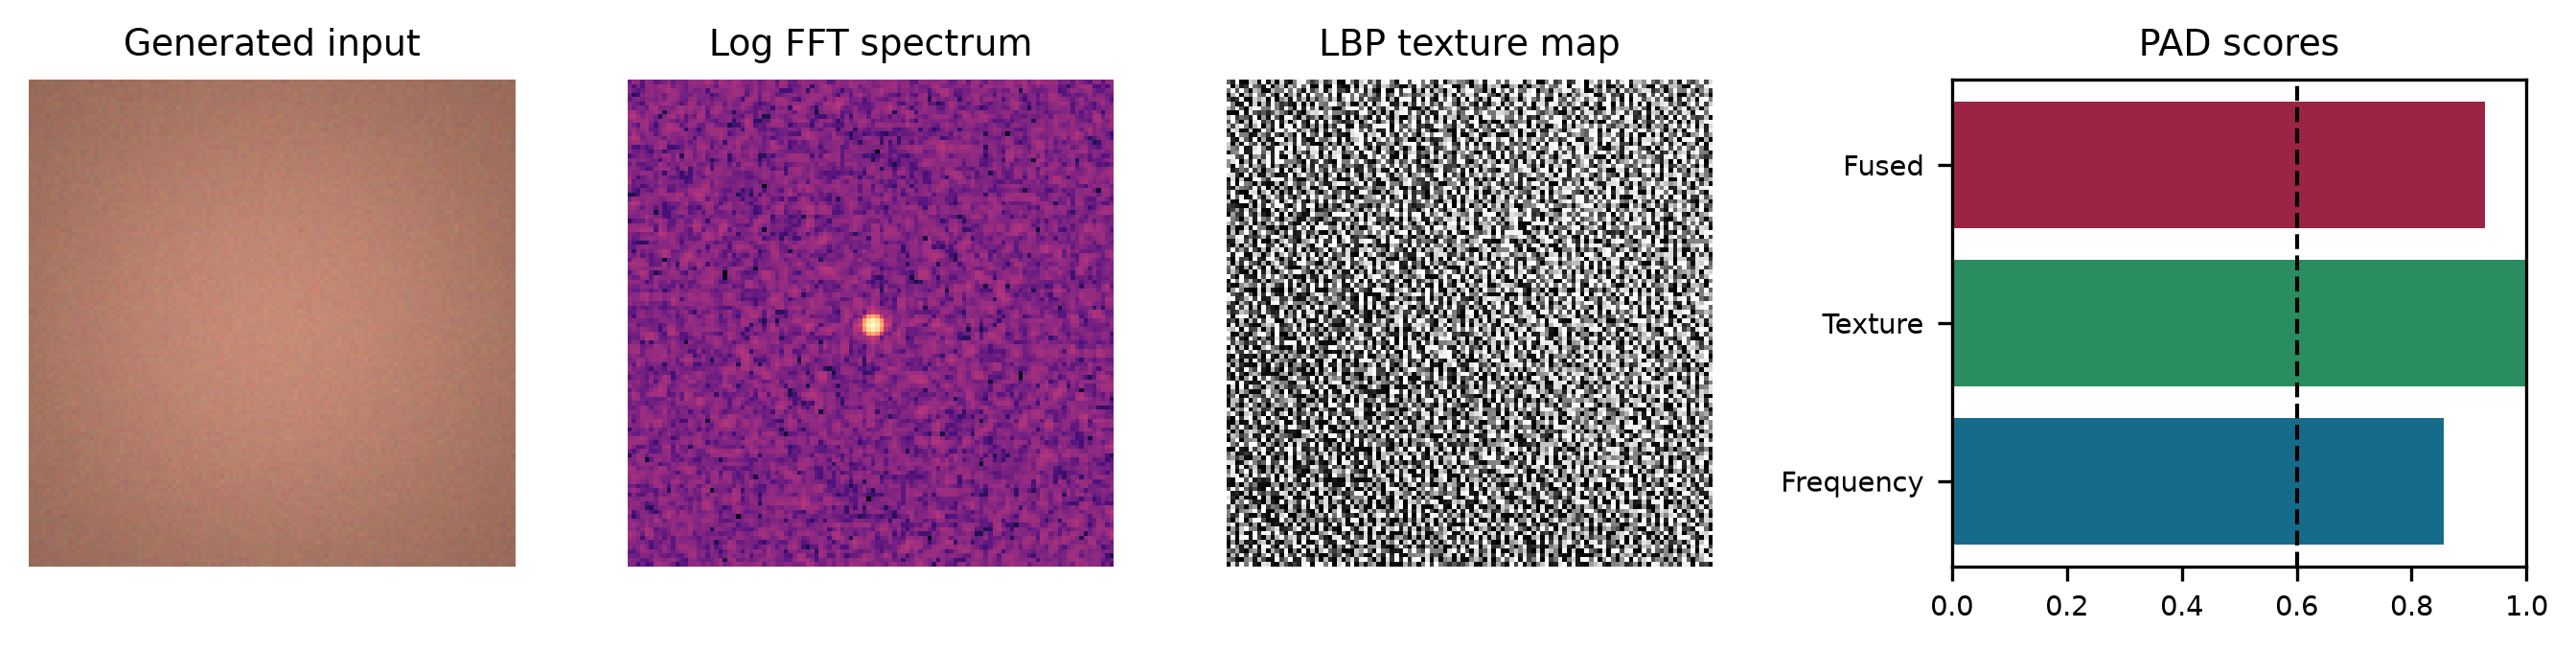
\includegraphics[width=0.91\textwidth]{figs/pad_diagnostics.png}
\caption{Generated input, its Fourier and LBP representations, and PAD scores. The dashed line marks the 0.60 decision threshold on the score panel. This is a synthetic illustration, not a camera-based PAD result.}
\label{fig:padvisual}
\end{figure*}

\begin{figure*}[t]
\centering
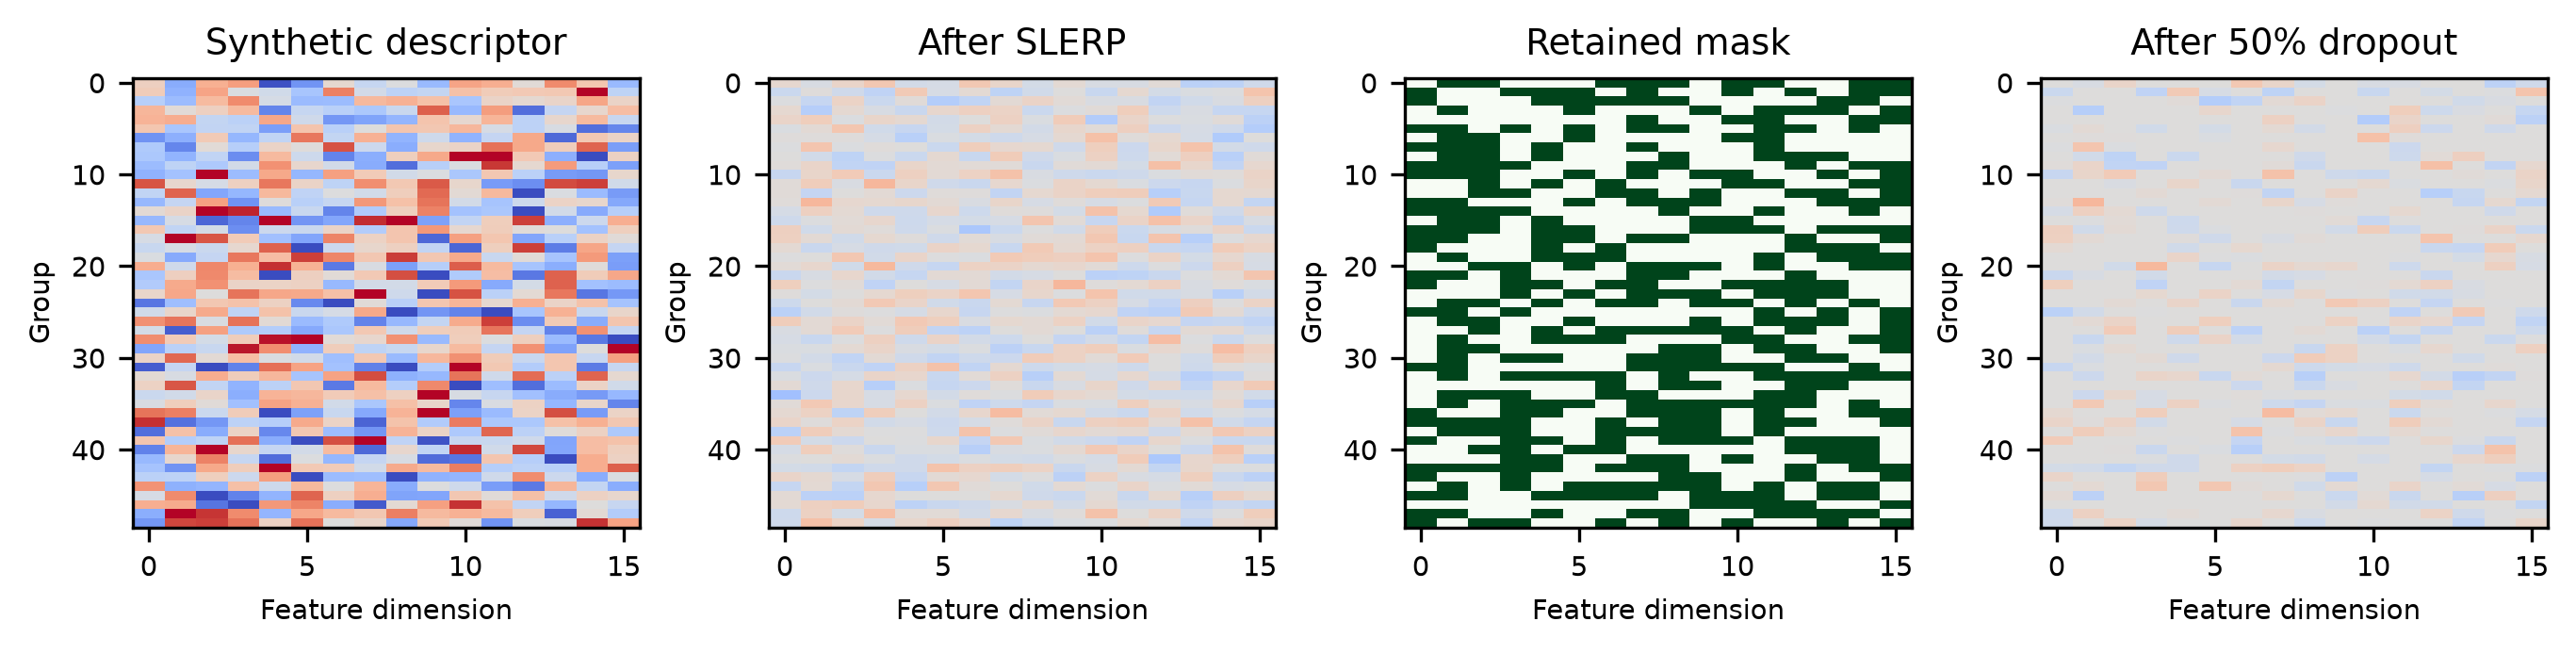
\includegraphics[width=0.91\textwidth]{figs/template_transform.png}
\caption{Synthetic grouped descriptor before SLERP, after SLERP, its retained-dimension mask, and after 50\% dropout. This illustration uses the implemented transform; resistance to reconstruction requires a separate attack evaluation.}
\label{fig:dropvisual}
\end{figure*}

\section{Experimental Setup}
\subsection{Controlled PAD Data}
The evaluation script uses NumPy seed 42 to generate 30 base images at $112\times112$ pixels. Each base produces one bona fide example, one simulated print, and one simulated screen presentation, for 90 images in total. The print generator compresses color range and adds a periodic halftone-like pattern; the screen generator adds periodic color modulation and a bright patch. These transformations are specified in the same repository as the PAD rules, so this experiment tests behavior on the project's own simulation rather than generalization to unseen attack devices.

Figure~\ref{fig:synthetic} shows one generated triplet. The base image is a smooth, skin-colored gradient, not a camera capture of a person's face. Here ``bona fide'' is the class name assigned by the generator rather than a verified live presentation. The simulated print and screen are transformations of that same base, making the three observations related. This design is useful as a deterministic software check, but it does not sample the diversity of real skin, faces, print materials, display pixels, camera sensors, or capture conditions.

\begin{figure*}[t]
\centering
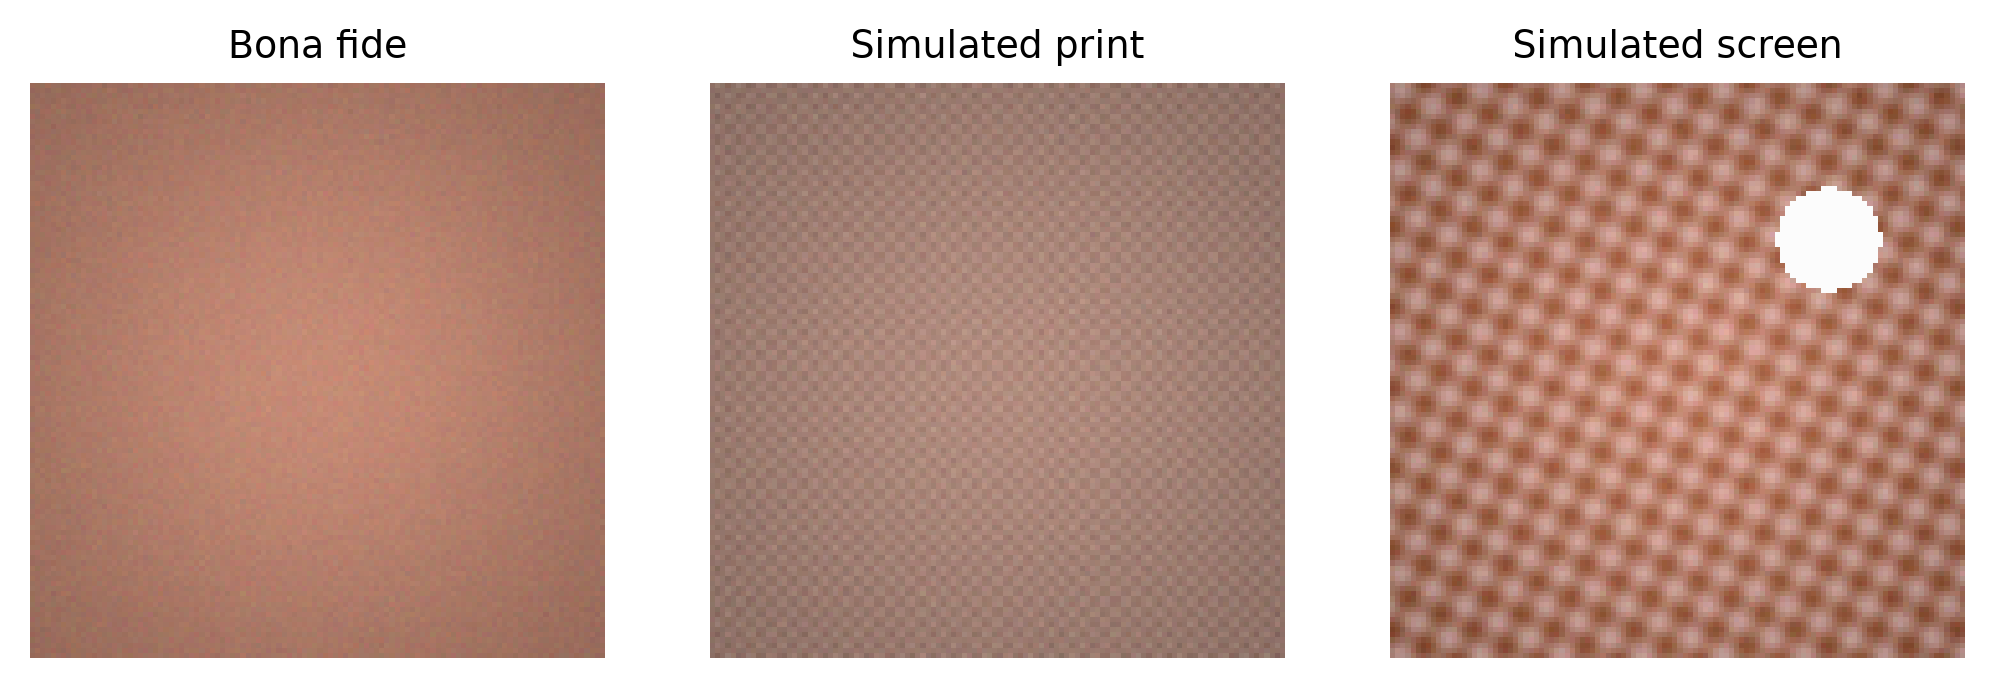
\includegraphics[width=0.90\textwidth]{figs/synthetic_triplet.png}
\caption{One generated test triplet from \texttt{evaluate\_antispoof.py}. The nominal genuine class is a colored gradient; print and screen artifacts are synthesized in software. The images are shown at the same scale to make the evaluation domain explicit.}
\label{fig:synthetic}
\end{figure*}

At the fixed liveness threshold of 0.60, we report bona fide presentation classification error rate (BPCER), attack presentation classification error rate (APCER), and their arithmetic mean, ACER:
\begin{equation}
\begin{aligned}
\mathrm{BPCER}&=N_{\mathrm{BR}}/N_{\mathrm{B}},\\
\mathrm{APCER}&=N_{\mathrm{AA}}/N_{\mathrm{A}},\\
\mathrm{ACER}&=(\mathrm{BPCER}+\mathrm{APCER})/2.
\end{aligned}
\label{eq:metrics}
\end{equation}
Here $N_{\mathrm{BR}}$ is the number of rejected nominal genuine samples, $N_{\mathrm{B}}$ the number of such samples, $N_{\mathrm{AA}}$ the number of accepted simulated attacks, and $N_{\mathrm{A}}$ the total attacks. The two simulated attack categories are pooled in the overall APCER denominator; their individual counts are also shown.

\subsection{Analysis Protocol}
We reran the original generator and detector without modifying their decisions. For each of the 90 examples, a separate analysis script records the final liveness score and the two component scores. It then constructs a class-wise score plot, a binary confusion matrix at the project's default threshold, and a threshold sweep from 0 to 1. The sweep reuses the same 90 scores and is descriptive; it is not an independent threshold-selection experiment. We also compare branch-score distributions to see which cues contribute to separation on these particular generated patterns. Since the branches have different hand-set scales and final penalties, that diagnostic is not a calibrated ablation study.

\subsection{Software and Timing Checks}
We ran the repository's 16-check comprehensive suite. It covers mathematical outputs, synthetic pairwise workflow cases, black and white input rejection, input-size handling, application syntax, and timing. Its speed check averages 30 calls to PAD on a bundled sample file, including file loading, and separately averages 30 template transformations on a dummy array. These are single-machine timings, not a controlled hardware comparison or a full camera-to-decision latency measurement.

\section{Results and Discussion}
\begin{figure*}[t]
\centering
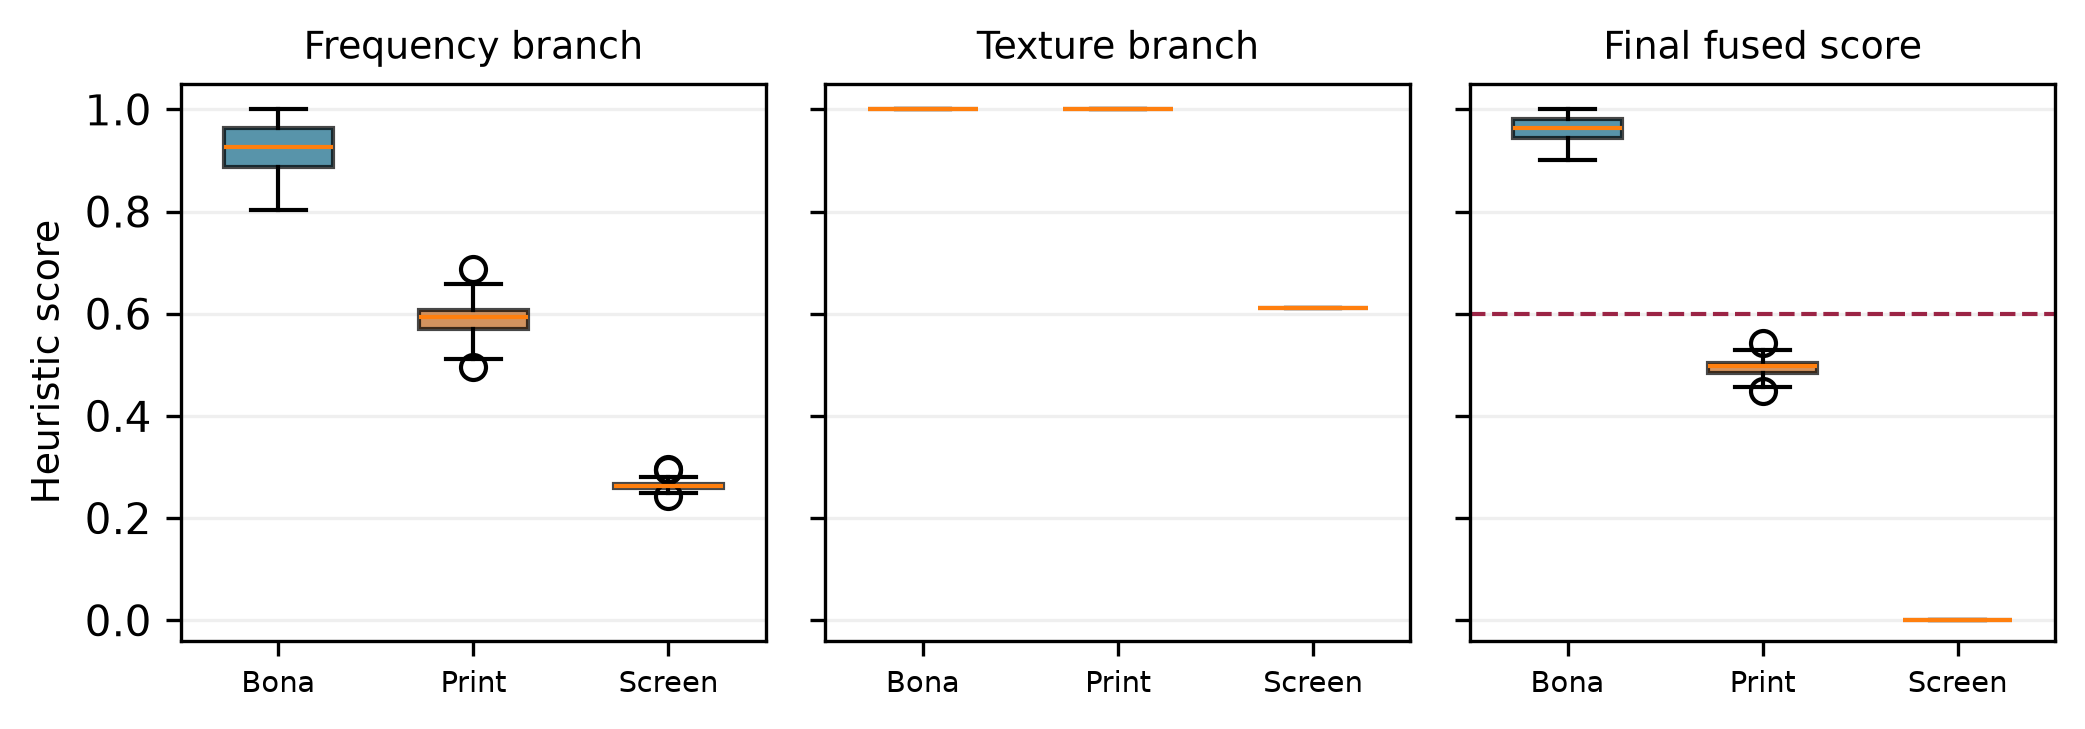
\includegraphics[width=0.91\textwidth]{figs/component_scores.png}
\caption{Branch and final score distributions for the generated data. The dashed line marks the decision threshold on the final score only; branch outputs are plotted as diagnostics and are not calibrated using that threshold.}
\label{fig:components}
\end{figure*}

\begin{table}[t]
\caption{PAD results on the 90-image generated test set at $L\geq0.60$}
\label{tab:padresults}
\centering
\footnotesize
\begin{tabular}{@{}lrrr@{}}
\toprule
Class & Images & Errors & Mean $L\pm$SD\\
\midrule
Bona fide & 30 & 0 rejected & $0.9612\pm0.0255$\\
Simulated print & 30 & 0 accepted & $0.4962\pm0.0217$\\
Simulated screen & 30 & 0 accepted & $0.0000\pm0.0000$\\
\midrule
Overall BPCER & 30 & \multicolumn{2}{c}{0/30 (0.00\%)}\\
Overall APCER & 60 & \multicolumn{2}{c}{0/60 (0.00\%)}\\
ACER & -- & \multicolumn{2}{c}{0.00\%}\\
\bottomrule
\end{tabular}
\end{table}

\subsection{PAD Scores and Binary Decisions}
Table~\ref{tab:padresults} shows no binary PAD errors on this generated set. Figure~\ref{fig:scoredist} adds the individual score positions and the $2\times2$ confusion matrix. All 30 nominal genuine samples scored at least 0.902; the highest simulated print score was 0.543 and all simulated screens were clipped to 0. The gap between the closest generated attack and genuine scores is therefore 0.358. At the default threshold of 0.60, the highest print score sits only 0.057 below the decision boundary. These are properties of the generated examples, not margins established for physical presentations.

\begin{figure*}[t]
\centering
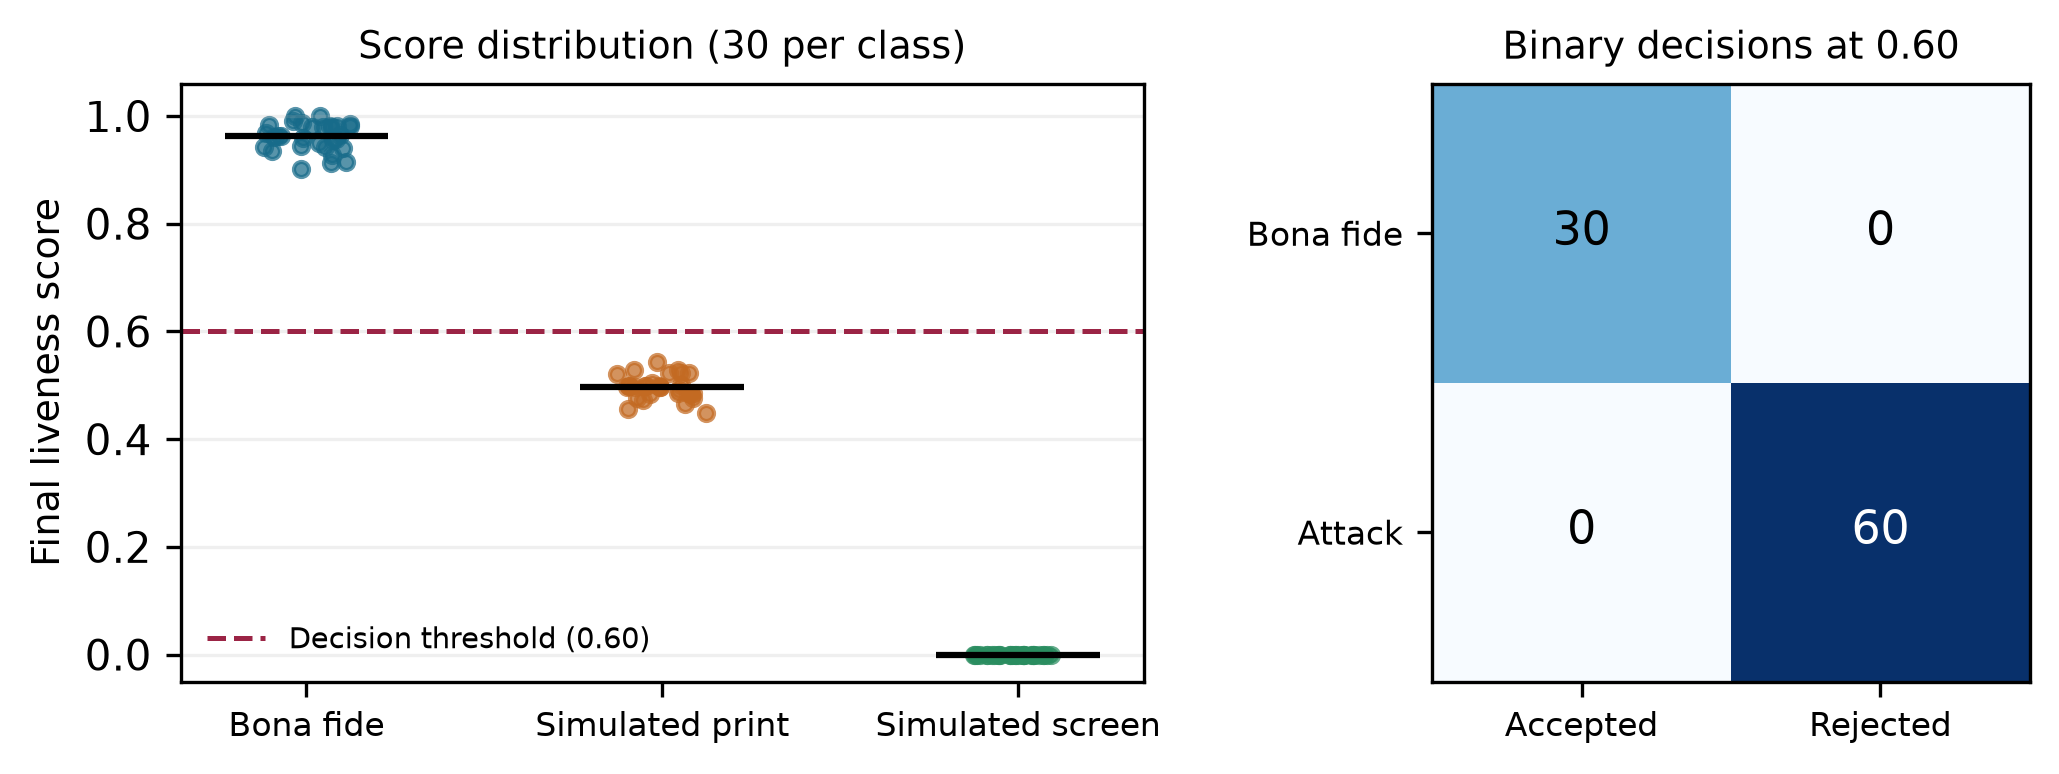
\includegraphics[width=0.91\textwidth]{figs/pad_score_and_confusion.png}
\caption{Left: all 90 final liveness scores, with median marks and the default decision threshold. Right: binary confusion matrix at 0.60. ``Attack'' pools the generated print and screen classes.}
\label{fig:scoredist}
\end{figure*}

This does not imply a zero error rate on photographs, physical printouts, screen replay videos, unfamiliar cameras, or different lighting. In particular, the screen examples have a conspicuous synthetic periodic modulation and bright hotspot; a real attack may have weaker or different cues. The 30 triplets also share their underlying generated base images, so the 90 rows should not be treated as 90 independent people or capture sessions. We report counts and descriptive score statistics rather than a population accuracy estimate.

\subsection{Threshold Sensitivity}
Figure~\ref{fig:threshold} and Table~\ref{tab:threshold} recompute decisions from the recorded scores at several thresholds. Lowering the threshold to 0.50 accepts 9 of 60 generated attacks. Raising it to 0.95 rejects 9 of 30 nominal genuine samples. On this particular set, thresholds above the maximum attack score (0.543) and at or below the minimum genuine score (0.902) yield no observed errors. That interval cannot be adopted as a deployment operating range without new, independently collected data. The project default, 0.60, was fixed in the evaluated script before this post-hoc sweep.

\begin{figure*}[t]
\centering
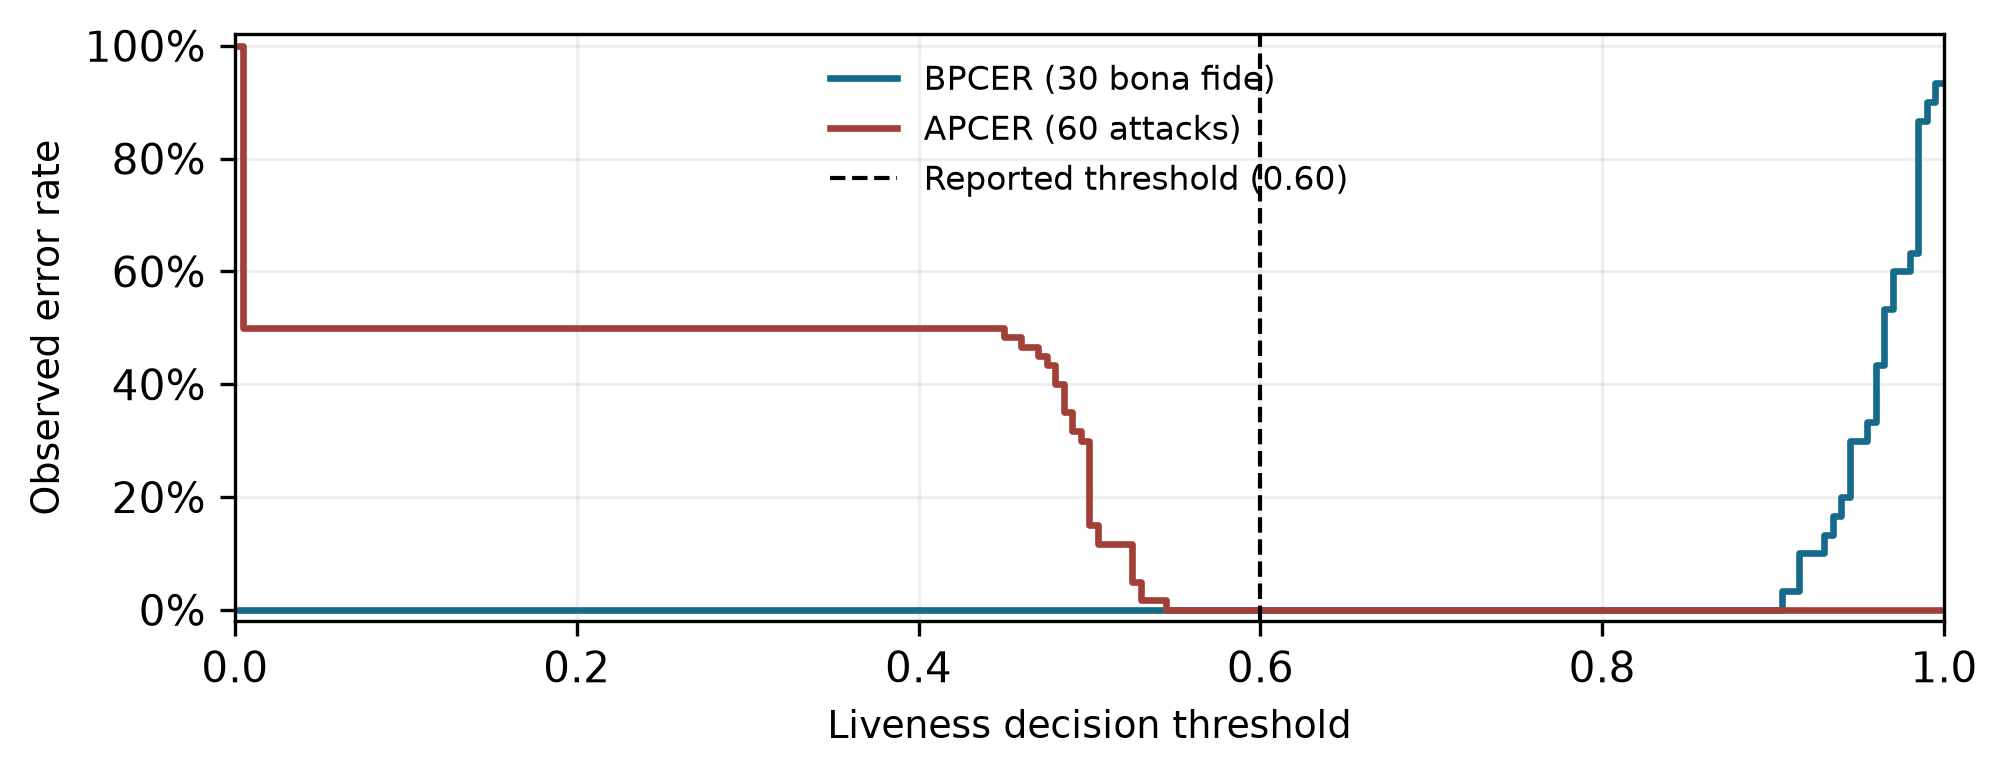
\includegraphics[width=0.86\textwidth]{figs/threshold_sensitivity.png}
\caption{Observed error rates when the decision threshold is varied on the same generated set. This is a sensitivity plot, not a held-out threshold calibration or a real-world detection error tradeoff curve.}
\label{fig:threshold}
\end{figure*}

\begin{table}[t]
\caption{Observed threshold sensitivity on the generated set}
\label{tab:threshold}
\centering\footnotesize
\begin{tabular}{@{}rrrr@{}}
\toprule
Threshold & Rej. /30 & Acc. /60 & ACER (\%)\\
\midrule
0.40 & 0 & 30 & 25.0\\
0.50 & 0 & 9 & 7.5\\
\textbf{0.60} & \textbf{0} & \textbf{0} & \textbf{0.0}\\
0.90 & 0 & 0 & 0.0\\
0.95 & 9 & 0 & 15.0\\
\bottomrule
\end{tabular}
\end{table}

\subsection{Frequency, Texture, and Fusion Diagnostics}
Table~\ref{tab:components} and Fig.~\ref{fig:components} compare the mean score from each PAD branch with the final fused decision. The generated print class receives a mean texture-branch score of 1.000, the same as the nominal genuine class. Its lower mean frequency score (0.592) and an additional 0.30 print-rule penalty reduce the final mean to 0.496. On these images, therefore, the texture branch alone is not what separates the simulated prints. The simulated screens have low frequency scores and a final score clipped to zero after fusion and penalties. This component analysis is useful for debugging the current rules, but the branch scores are not separately calibrated classifiers.

\begin{table}[t]
\caption{Mean heuristic scores by generated class ($n=30$ each)}
\label{tab:components}
\centering\footnotesize
\begin{tabular}{@{}lrrr@{}}
\toprule
Class & Frequency & Texture & Final\\
\midrule
Nominal genuine & 0.922 & 1.000 & 0.961\\
Simulated print & 0.592 & 1.000 & 0.496\\
Simulated screen & 0.264 & 0.611 & 0.000\\
\bottomrule
\end{tabular}
\end{table}

\subsection{Workflow and Timing Checks}

The comprehensive suite passed 16/16 checks in the local run. Its measured average PAD time was 17.42 ms per sample (approximately 57.4 calls/s), and its average SLERP transformation time was 0.222 ms per template. These values differ from faster figures recorded in older project notes; execution environment and timing scope can affect them. The workflow checks established that synthetic spoof inputs exited before feature extraction in the tested calls. They did not test storage, network transmission, or an adversarial attempt to bypass the gate.

\subsection{Fallback Matching Sanity Check}
The bundled examples include two images labeled synthetic person A and one labeled synthetic person B. We extracted the fallback descriptors, applied the same seeded SLERP and dropout operation used by the CLI, and calculated cosine similarity. Table~\ref{tab:matching} shows that the nominal different-person pair also exceeds the project's 0.30 match threshold. All three bundled images pass the PAD gate with a score of 0.70, so PAD would not prevent this particular identity mismatch. This is a small diagnostic on generated examples, not a false-match-rate estimate across people.

\begin{table}[t]
\caption{Fallback-descriptor similarity on bundled synthetic examples}
\label{tab:matching}
\centering\footnotesize
\setlength{\tabcolsep}{4pt}
\begin{tabular}{@{}lrrc@{}}
\toprule
Pair & Raw cosine & Protected cosine & $\geq0.30$?\\
\midrule
A1--A2 (same label) & 0.9999 & 1.0000 & Yes\\
A1--B1 (different label) & 0.9961 & 0.9999 & Yes\\
\bottomrule
\end{tabular}
\end{table}

The comprehensive suite checks that A1--A2 is accepted and that the two generated attack images are stopped by PAD; it does not assert that A1--B1 is rejected. The nearly identical similarity scores show why the fallback descriptor must not be treated as a validated face recognizer. Since the trained IR-50 checkpoint is unavailable in this checkout, no result here measures recognition with the trained SlerpFace backbone. Likewise, the shape and sparsity of the protected template do not prove irreversibility, unlinkability, or resistance to a diffusion-based inversion attack. Those questions require a separate attack and identity evaluation under specified key conditions.

\balance
\section{Limitations and Future Work}
\subsection{Physical PAD Evaluation}
The PAD logic is hand-tuned and the present benchmark is generated by the same codebase. The synthetic gradient triplets reveal that 0\% observed error here is principally a software sanity check. A physical study should collect consented direct camera captures and attacks made from printed images and displayed images. It should vary the source subjects, printers, paper types, displays, cameras, viewing distances, pose, ambient light, and screen brightness. Every test record should identify the attack instrument and capture conditions. In particular, a screen shown to a webcam may not reproduce the exact periodic pattern injected by the current generator.

Calibration and reporting sets should be disjoint by subject and, where feasible, by attack instrument. The liveness threshold and any rule weights should be fixed using calibration data, then evaluated once on held-out data. Report APCER separately for print and screen subtypes, BPCER across genuine capture conditions, and the denominators behind each rate. A detection-error tradeoff curve can be reported for the held-out set if the score is stable enough to sweep; a single 0.60 operating point alone does not show the acceptance/rejection tradeoff. The implementation also needs an explicit face-detection and alignment stage, since the current PAD path processes the supplied RGB image as a whole. A motionless face video, mask, and injected digital image represent additional threats that this static-image experiment has not tested.

\subsection{Recognition and Template Privacy}
For face verification, the trained backbone checkpoint and a labeled identity dataset are prerequisites. A proper trial list would separate enrollment and probe images, include many mated and non-mated pairs, and choose the protected-match threshold on a development split. Results should then include false-match and false-nonmatch rates, as well as accuracy at stated operating points. The A1--B1 result in Table~\ref{tab:matching} shows why the fallback descriptor and the default 0.30 threshold cannot substitute for that evaluation. The same pair list should be measured before and after protection so that any recognition cost is attributable to the transformation under a fixed feature extractor.

The fixed demo seed should be replaced with a specified key-management design before claims of cancelability or cross-system unlinkability. The original SlerpFace paper studies these properties with its own model and key assumptions~\cite{slerpface}; repeating its equation in the CLI does not transfer those empirical guarantees. A local privacy evaluation would require protected templates, explicit attacker knowledge, an inversion method, a reconstruction metric, and a cross-system linking experiment with different keys. The present figures verify only the form of the transformed array and the exact number of zeroed elements.

\subsection{System Boundary}
The current early return prevents feature extraction inside the tested call when PAD rejects an image. It does not establish that a deployed camera stack, application logs, network path, or database never handles unprotected face data. Those components are outside the repository's controlled benchmark. Once a complete application boundary exists, tracing data from capture through storage and deletion would be needed to validate an end-to-end handling claim. The current report therefore treats the early return as an implemented control-flow property and keeps broader operational security as future work.

\section{Conclusion}
GuardFace demonstrates a clear software integration: a PAD decision precedes feature extraction and SlerpFace-style grouped template transformation. The locally rerun generated-image benchmark produced no PAD errors among 90 examples, and the repository's 16 checks passed. The different-label bundled pair was nevertheless accepted by the fallback matcher, showing that the present checkout does not support a face-recognition accuracy claim. Physical PAD performance, trained-backbone face verification, and template privacy remain open empirical questions for the next evaluation phase.

\begin{thebibliography}{4}
\bibitem{slerpface} Z. Zhong \emph{et al.}, ``SlerpFace: Face template protection via spherical linear interpolation,'' \emph{Proc. AAAI Conf. Artificial Intelligence}, vol. 39, no. 10, pp. 10698--10706, 2025, doi: 10.1609/aaai.v39i10.33162.
\bibitem{ojala} T. Ojala, M. Pietik\"ainen, and T. M\"aenp\"a\"a, ``Multiresolution gray-scale and rotation invariant texture classification with local binary patterns,'' \emph{IEEE Trans. Pattern Anal. Mach. Intell.}, vol. 24, no. 7, pp. 971--987, 2002, doi: 10.1109/TPAMI.2002.1017623.
\bibitem{iso30107} ISO/IEC 30107-3:2023, \emph{Information technology---Biometric presentation attack detection---Part 3: Testing and reporting}, 2nd ed., 2023. [Online]. Available: \url{https://www.iso.org/standard/79520.html}
\bibitem{guardfacecode} GuardFace project team, ``SlerpFace IEEE Extend: GuardFace project repository,'' GitHub. [Online]. Available: \url{https://github.com/neev-25/SlerpFace_IEEE_Extend}. Accessed: Sep. 23, 2026.
\end{thebibliography}

\end{document}
